\documentclass{article}
\newcommand{\hwnumber}{1}

\newcommand{\norm}[1]{\| #1 \|}
\newcommand{\abs}[1]{| #1 |}

\usepackage{fullpage,amsthm,amsmath,amssymb}
\usepackage{algorithm,algorithmic}
\usepackage{mathtools}
\usepackage{bbm,bm}
\usepackage{enumerate}
\usepackage{xspace}
\usepackage{tikz}
\usepackage{graphicx}
\usetikzlibrary{positioning}
\usepackage[textsize=tiny,
]{todonotes}
\newcommand{\todot}[1]{\todo[color=blue!20!white]{T: #1}}
\newcommand{\todoc}[1]{\todo[color=orange!20!white]{Cs: #1}}
\usepackage[colorlinks,citecolor=blue,urlcolor=blue,linkcolor=black]{hyperref}
\newcommand\numberthis{\addtocounter{equation}{1}\tag{\theequation}}

\newtheorem{theorem}{Theorem}
\newtheorem{corollary}{Corollary}

\newcommand{\R}{\mathbb{R}}
\DeclareMathOperator*{\argmin}{argmin}
\DeclareMathOperator{\sign}{sign}
\DeclareMathOperator{\Var}{Var}
\DeclareMathOperator{\Lap}{Lap}
\DeclareMathOperator*{\Exp}{\mathbf{E}}
\DeclareMathOperator*{\1}{\mathbbm{1}}
\newcommand{\set}[1]{\left\{#1\right\}}
\newcommand{\E}{\mathbb E}
\newcommand{\V}{\mathbb V}
\renewcommand{\P}[1]{P\left\{ #1 \right\}}
\newcommand{\Prob}[1]{\mathbb{P}( #1 )}
\newcommand{\real}{\mathbb{R}}
\renewcommand{\b}[1]{\mathbf{#1}}
\newcommand{\EE}[1]{\E[#1]}
\newcommand{\bfone}{\1}
\newcommand{\NN}{\mathbb{N}}
\newcommand{\cF}{\mathcal{F}}
\newcommand{\w}{\textbf{w}}
\newcommand{\x}{\textbf{x}}
\newcommand{\X}{\textbf{X}}
\newcommand{\y}{\textbf{y}}
\newcommand{\z}{\textbf{z}}
\newcommand{\f}{\textbf{f}}
\newcommand{\g}{\textbf{g}}
\newcommand{\D}{Diag}
\newcommand{\In}{\mathbf{I}_n}
\newcommand{\one}{\textbf{1}}
\newcommand{\qedwhite}{\hfill \qed}
\usepackage[capitalize]{cleveref}
\usepackage{xifthen}

\newcounter{DocPoints} 
\newcounter{QuestionPoints} 
\newcommand{\points}[1]{	\par\mbox{}\par\noindent\hfill {\bf #1 points}	\addtocounter{DocPoints}{#1}
	\addtocounter{QuestionPoints}{#1}
}
\newcommand{\tpoints}[1]{        	\ifthenelse{\isempty{#1}}	{	}	{		\addtocounter{DocPoints}{#1}
		\addtocounter{QuestionPoints}{#1}
	}													 	\par\mbox{}\par\noindent\hfill {Total: \bf \arabic{QuestionPoints}\xspace points}\par\mbox{}\par\hrule\hrule
	\setcounter{QuestionPoints}{0}
}
\newcommand{\tpoint}[1]{
	\tpoints{#1}
}

\theoremstyle{definition}
\newtheorem{question}{Question}

\theoremstyle{remark}
\newtheorem{remark}{Remark}
\newtheorem*{remark*}{Remark}
\newtheorem{solution}{Solution}
\newtheorem*{solution*}{Solution}

\newcommand{\hint}{\noindent \textbf{Hint}:\xspace}

\usepackage{hyperref}

\newcommand{\epssub}{\delta}
\newcommand{\cH}{\mathcal{H}}
\newcommand{\sA}{\mathcal{A}}
\newcommand{\cS}{\mathcal{S}}
\newcommand{\cA}{\mathcal{A}}
\newcommand{\cB}{\mathcal{B}}
\newcommand{\vecf}{\mathbf{f(x)}}

\begin{document}

\section*{Question 1}
\section*{1.1}
\large
\begin{align*}
    \nabla_b \sum_i(x_i-b)^2 = 0
    & \Rightarrow 2 \sum_i (x_i - b) = 0 \\
    &\Rightarrow \sum_i x_i - nb = 0 \\ 
    & \Rightarrow \sum_i x_i = nb \\
    & \Rightarrow \boxed{ b = \frac{1}{n} \sum_i x_i}
\end{align*}        
\section*{1.2}
The optimal value for b is the average of a normal distribution
\section*{1.3}
The minimum value for this loss function is going to be 0, because of the 
absolute value.
\begin{align*}
 \sum_i \abs{x_i - b} = 0 \Rightarrow \boxed{b = \frac{1}{n} \sum_i x_i}
\end{align*}
\section*{Question 2}
 Linear function of a column vector $[x_1,x_2,...,1]^T$, can be expressed as a linear transformation:
 \begin{align*}
    f(\x) = \x^T\w + b = [\x, \, 1][\w, \, b]^T
 \end{align*}

\section*{Question 3}

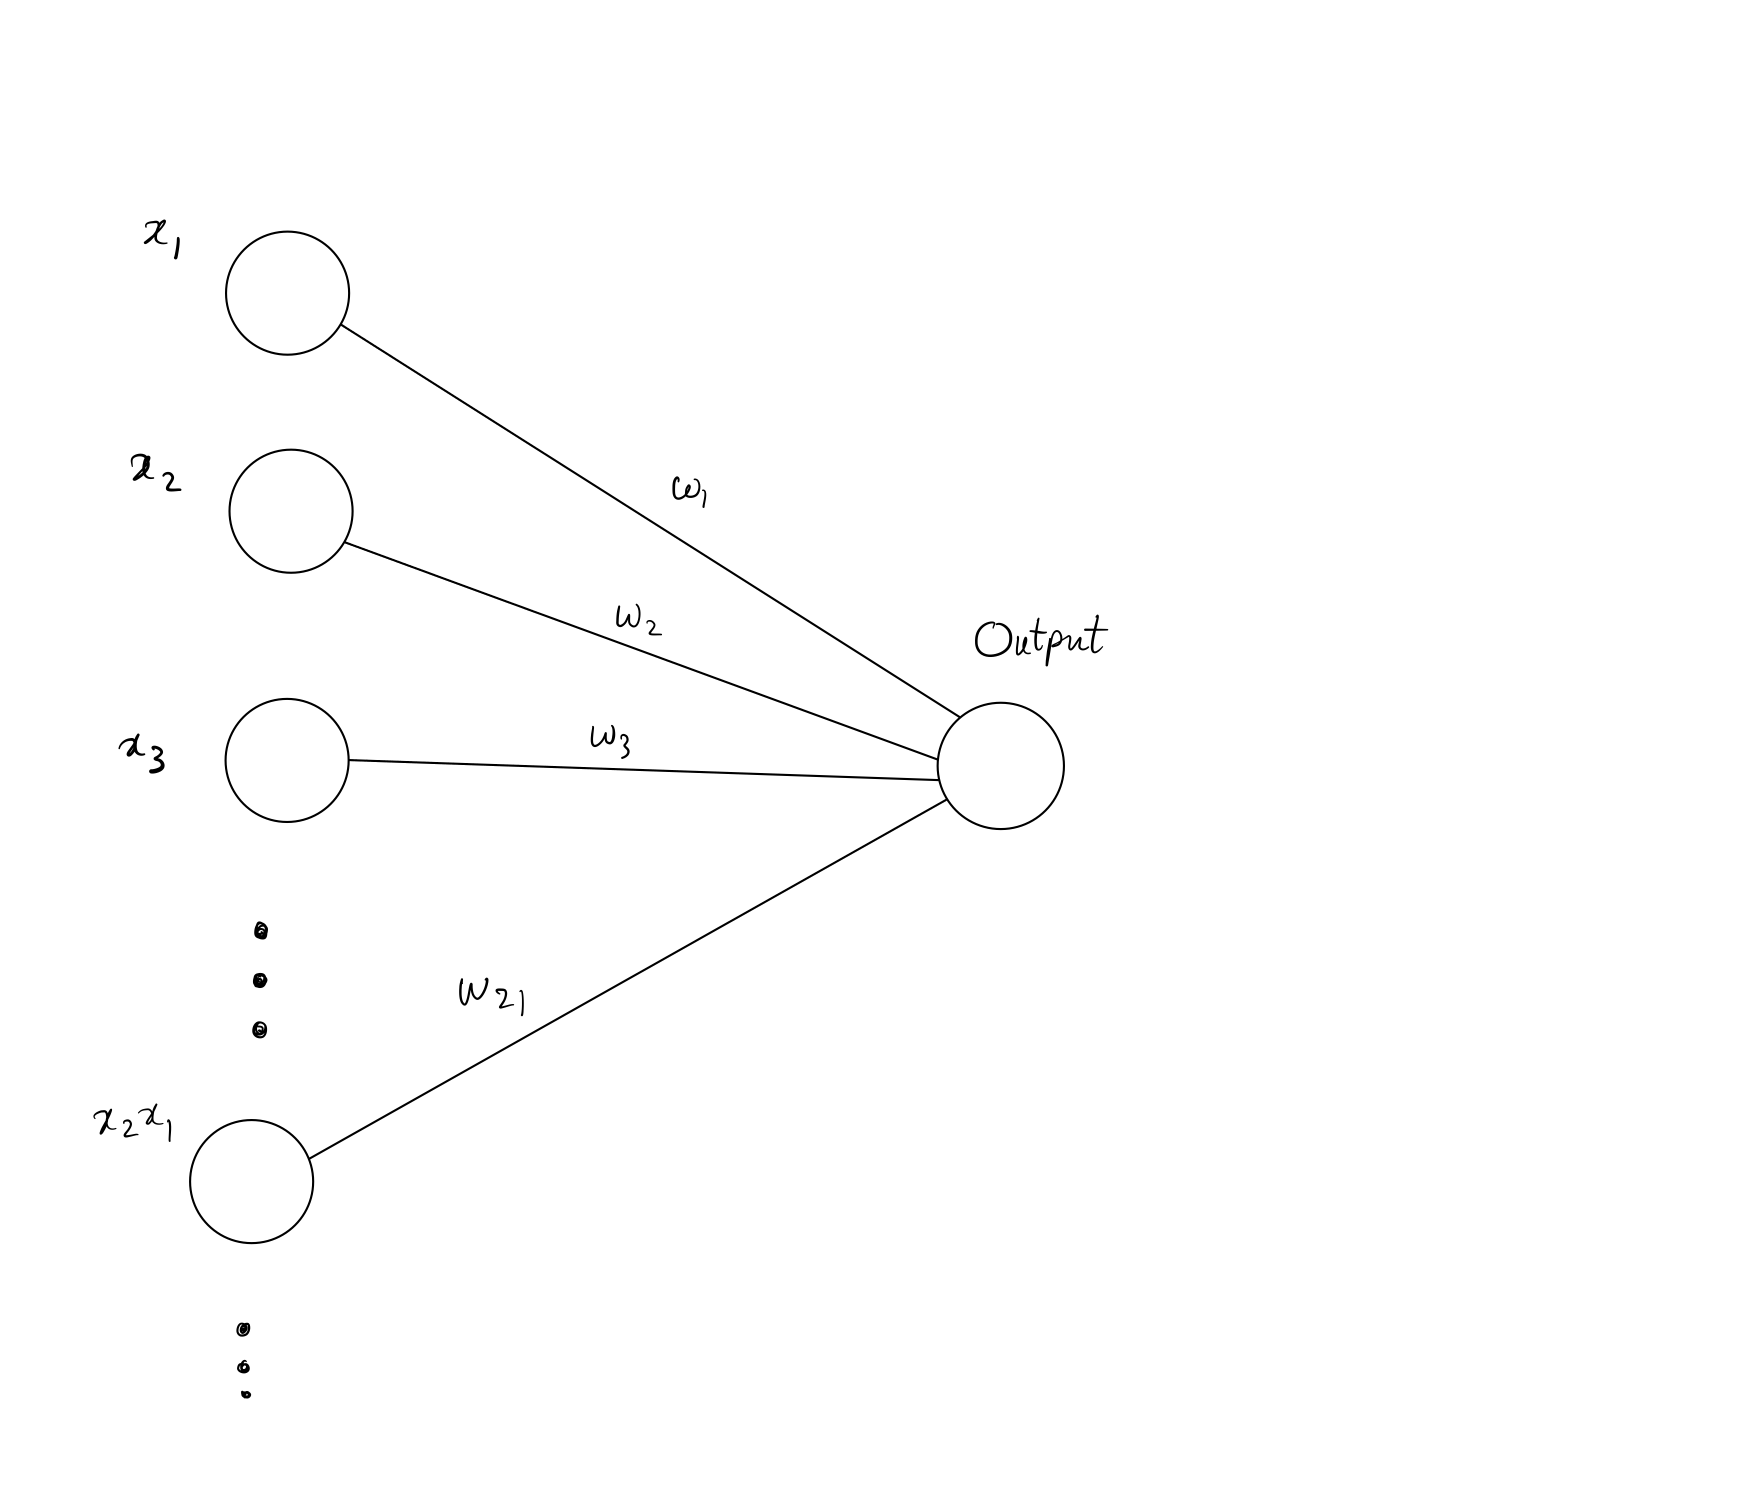
\includegraphics[width=0.8\linewidth]{NN.png}

\section*{Question 4}
\section*{4.1}
The matrix $\textbf{X}^T\textbf{X}$ won't be invertible. Thus, no unique solution 
will exist for the optimal weight $\w^*$.
\section*{4.2}
One way to potentially fix it is to use a technique to approximate the inverse of $\textbf{X}^T\textbf{X}$.
Introducing noise will do the following:\\
\begin{align*}
    (\textbf{X} + \mathbf{\epsilon})^T(\textbf{X} + \mathbf{\epsilon})
    & = \textbf{X}^T\textbf{X} + \textbf{X}^T\mathbf{\epsilon} 
    + \mathbf{\epsilon}^T\textbf{X} + \mathbf{\epsilon}^T\mathbf{\epsilon} 
\end{align*}
where $\mathbf{\epsilon}$ is a matrix of all noise entries.
\section*{4.3}
\begin{align*}
    \E[ \textbf{X}^T\textbf{X} + \textbf{X}^T\mathbf{\epsilon} 
+ \mathbf{\epsilon}^T\textbf{X} + \mathbf{\epsilon}^T\mathbf{\epsilon}] \\
= \E[ \textbf{X}^T\textbf{X}] + \E[\textbf{X}^T\mathbf{\epsilon}]
+ \E[\mathbf{\epsilon}^T\textbf{X}] + \mathbf{\epsilon}^T\mathbf{\epsilon}
\end{align*}
\section*{4.4}
The SGD algorithm is unable to find a global minimum.
\section*{Question 5}
\section*{5.1}
\begin{align*}
    - \log P(\y|\X) = \sum_i\abs{y - \w^Tx^{(i)} - b}
\end{align*}
\section*{5.2}
Unable to provide closed form solution.
\section*{5.3}
I think using the standard minibatch SGD update is sufficient:
\begin{align*}
 \w \leftarrow \w - \frac{\eta}{\abs{\beta}} \sum_i \x^{(i)}(\w^T\x^{(i)} + b - y^{(i)})  
\end{align*}
\section*{Question 6}
It doesn't work because it needs at least one more layer as the final output layer.
\section*{Question 7}
To be added...
\section*{Question 8}
To be added...
\end{document}
